\section{Requirements Captured}
The next section deals with the analysis of your system. Cover the
functional, non-functional and usability requirements. This is where
you present your use case narratives and diagrams. 

Discuss the major analysis artefacts that you produced. We will expect
you to produce at least one overall description of the architecture
used in your system as a diagram, either here or below (see Section
\ref{ss:design-overview}). You may also want to include an analysis
class hierarchy diagram.

\subsection{Design Overview}
\label{ss:design-overview}

The next section is an overview of your design. The system design has
to be justified in terms of the expected behaviour of the final
product. 

If you produced a design class diagram put it here.

\begin{figure}[h!]
  \center{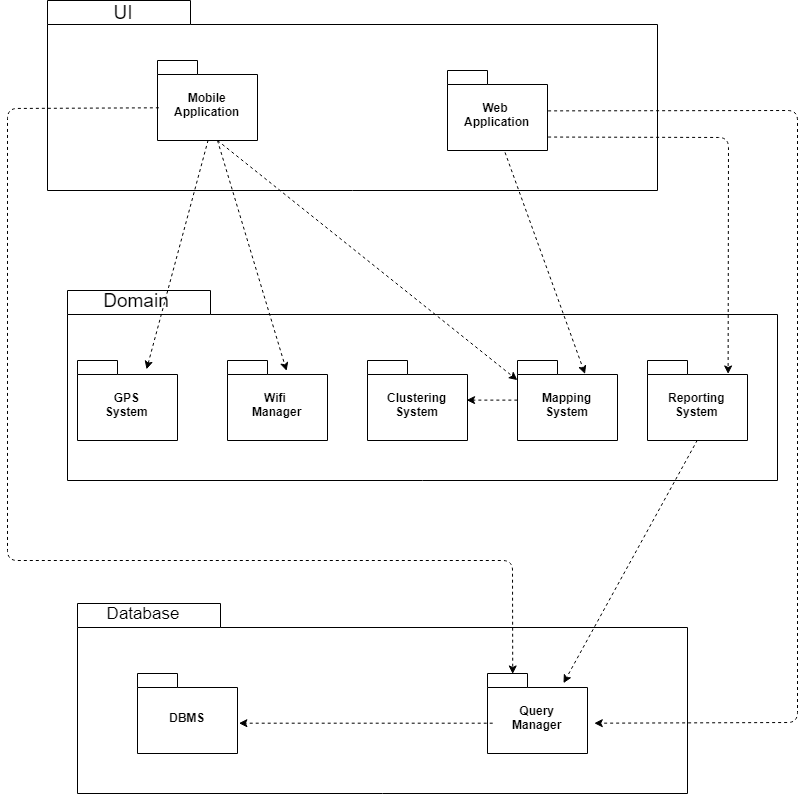
\includegraphics[scale=0.8]{images/architecture.png}}
  \caption{An architecture diagram. Caption to go below figure}
  \label{fig:architecture}
\end{figure}

You must present the overall architecture of the system together with
an architecture diagram. You may choose what kind of diagram best
suits your project but we would expect a layered architecture diagram
(see Figure \ref{fig:architecture}) unless there is a good reason for
some other kind of diagram. It need not be a formal UML diagram as
long as it conveys all the necessary information clearly.

You should then (in subsections) cover the algorithms and the data
organisation used and why they were considered the best. 

